\chapter{Results and discussion}
\label{results}
Summarise the results...

\section{Data collection}
\label{results:collection}
Brazil, Mexico and India have been chosen for this experiment as Tinder is very
popular in these countries \citep{tinderPopular} and have much smaller
proportions of immigrant population compared to other countries in which Tinder
is popular such as the United States and the United Kingdom
\citep{desa2013trends}.

Using the state-of-art race recognition algorithms faces from Brazil and Mexico
would be classified as Hispanic so it would be interesting to see how well it
is possible to split this single class further. 

A non-capital city was chosen in each of the three countries and the data
collection service was tasked with setting its own location to those cities one
at a time and collecting pictures from local profiles for several days. The
breakdown of images collected per gender and location is summarised in
\Cref{table:results:dc:total_images}.
\begin{table}[t]
    \begin{center}
        \begin{tabular}{ c c c c c }
            \toprule
            Country       & City              & Male   & Female & Total \\ 
            \toprule
            Brazil  & Belo Horizonte &  4090 & 9688 & 13778\\
            India   & Mumbai         &  5014 & 3607 & 8621 \\
            Mexico  & Guadalajara    &  4887 & 3861 & 8748\\
            \bottomrule
        \end{tabular}
    \end{center}
    \caption{Total images collected by location and gender}
    \label{table:results:dc:total_images}
\end{table}

\section{Face and landmark detection}
\label{results:fd}
Images collected in the previous stage were passed through the face detection
stage to determine the presence of one or more faces and estimate the locations
of key facial landmarks. On average, the algorithm took around $6.5$ seconds to
perform face detection in a single image. Due to this limitation it was not
possible to detect faces in all images collected, however it was ensured that
at least 3000 images per location and gender passed through the face detection
stage. The actual numbers of images in which face detection was attempted can
be seen in \Cref{table:results:fd:detected}.
\begin{table}[t]
    \begin{center}
        \begin{tabular}{ c c c c}
            \toprule
            Country       & City              & Male   & Female\\ 
            \toprule
            Brazil  & Belo Horizonte &  3303 (81\%) & 6193 (64\%)\\
            India   & Mumbai         &  3771 (75\%) & 3149 (87\%)\\
            Mexico  & Guadalajara    &  3230 (66\%) & 3650 (95\%)\\
            \bottomrule
        \end{tabular}
    \end{center}
    \caption{Numbers and percentages of images passed through the face
    detection stage. Images in which there were no faces detected also
contribute to the numbers.}
    \label{table:results:fd:detected}
\end{table}

\begin{figure}
    \centering
    \begin{subfigure}[b]{0.3\textwidth}
      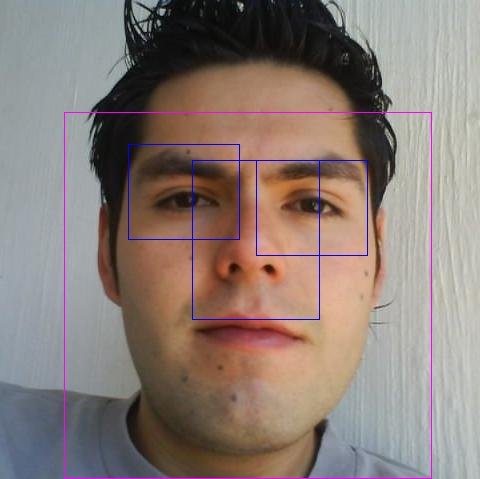
\includegraphics[width=\textwidth]{figures/results/detected_cff0618f-f631-4b0d-80d9-f582fee46fad}
      \caption{Score=1.4313}
      \label{fig:results:fd:good_detected1}
    \end{subfigure}
    \begin{subfigure}[b]{0.3\textwidth}
      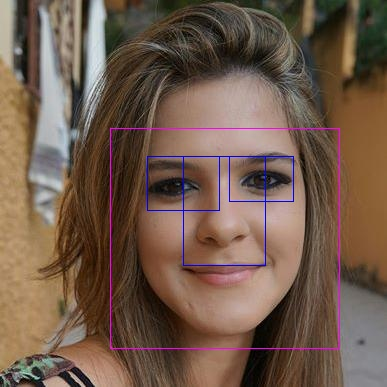
\includegraphics[width=\textwidth]{figures/results/detected_50508cb1-814e-4374-bf07-cef5c301c3c0}
      \caption{Score=1.20387}
      \label{fig:results:fd:good_detected2}
    \end{subfigure}
    \begin{subfigure}[b]{0.3\textwidth}
      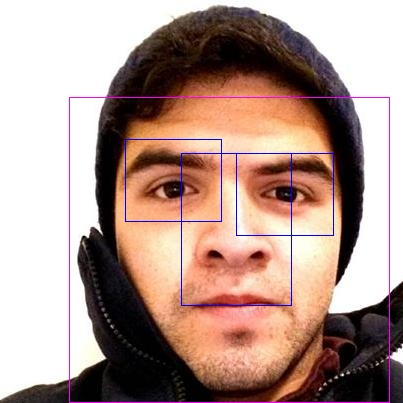
\includegraphics[width=\textwidth]{figures/results/detected_da153846-1afe-4b36-880a-bf8764bfd935}
      \caption{Score=1.09232}
      \label{fig:results:fd:good_detected3}
    \end{subfigure}
\caption{Three examples of high-scoring face detections.}
\label{fig:results:fd:good_detected}
\end{figure}

\begin{figure}
    \centering
    \begin{subfigure}[t]{0.3\textwidth}
      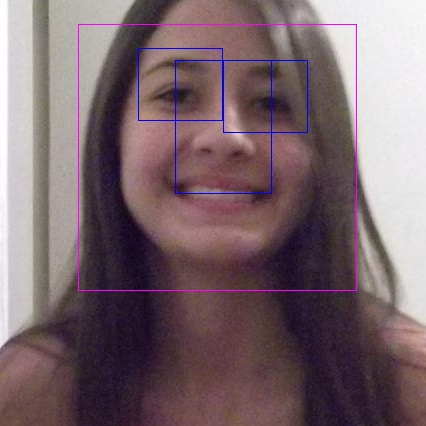
\includegraphics[width=\textwidth]{figures/results/detected_q3_15c3f02d-31c6-4955-8d05-c05029cdb473}
      \caption{Face detection with score=0.0651244 in upper quartile}
      \label{fig:results:fd:q3_detected2}
    \end{subfigure}
    \begin{subfigure}[t]{0.3\textwidth}
      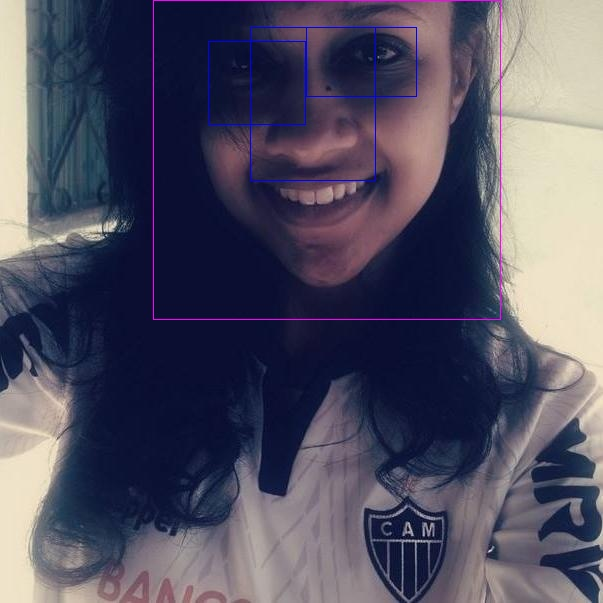
\includegraphics[width=\textwidth]{figures/results/detected_median_fcb1d3ed-7867-40ba-9691-8cd1f59dc36b}
      \caption{Face detection with score=-0.108765 around the median}
      \label{fig:results:fd:median_detected1}
    \end{subfigure}
    \begin{subfigure}[t]{0.3\textwidth}
      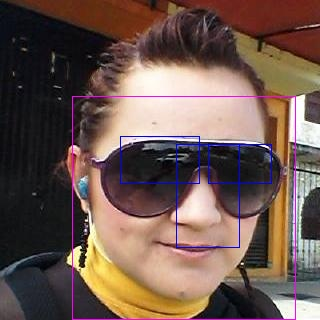
\includegraphics[width=\textwidth]{figures/results/detected_q1_f1c5f486-1697-4089-9bb6-7962d7db630c}
      \caption{Face detection with score=-0.517613 in lower quartile}
      \label{fig:results:fd:q1_detected3}
    \end{subfigure}
\caption{Examples of inferior face pictures. Cropped foreheads, blurriness, sunglasses and small faces are some obvious reasons why a face detection might have received a low score.}
\label{fig:results:fd:other_detected}
\end{figure}

\begin{figure}
    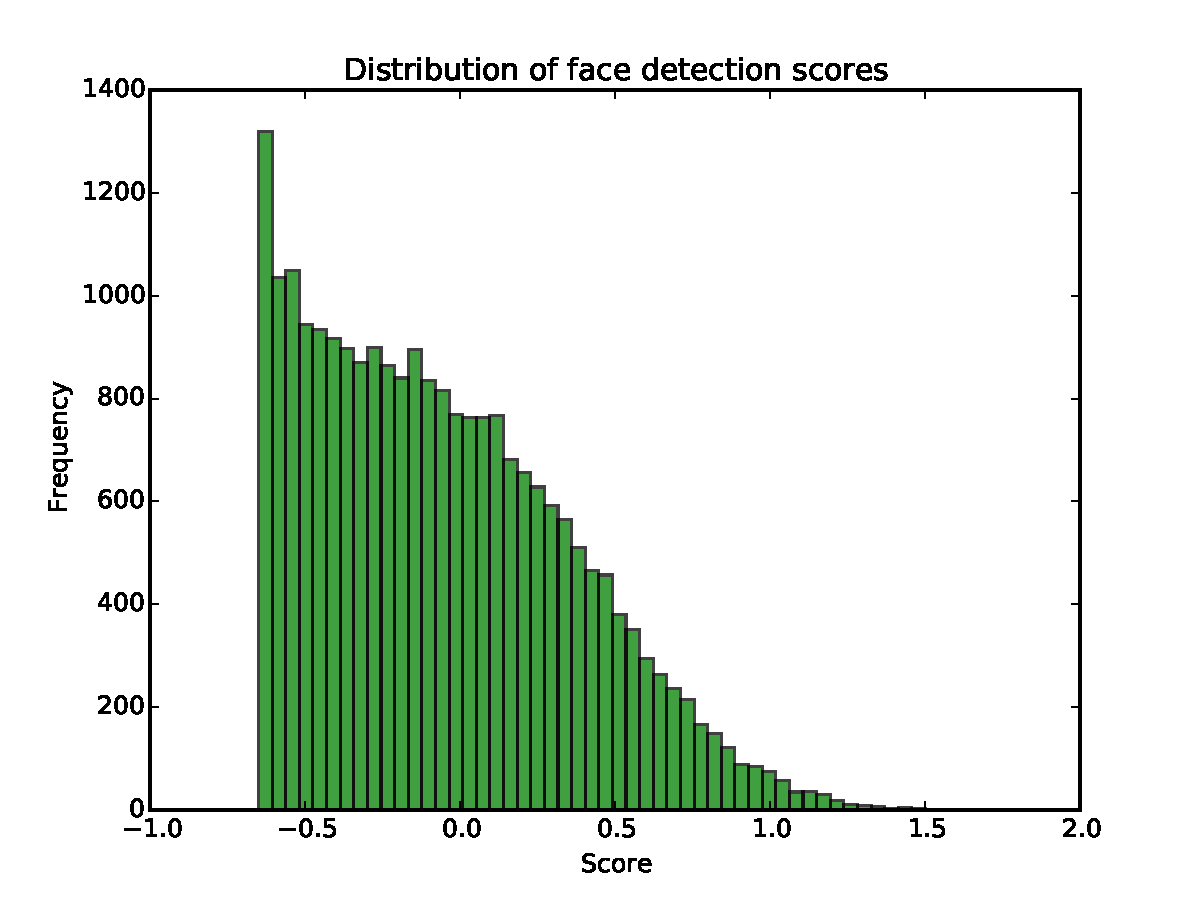
\includegraphics[width=\textwidth]{figures/results/scores_hist}
    \caption{Histogram of scores given by the face detection algorithm to 23379 images.}
    \label{fig:results:fd:scores_hist}
\end{figure}

\section{Data analysis and classification}
\begin{table}[b]
      \centering
      \begin{tabular}{l c c c}
        \toprule
        &                    India(predicted)                 & Brazil(predicted)          & Mexico(predicted) \\
        \midrule
        India(actual)              & 0.62                     & 0.18                       & 0.2 \\
        Brazil(actual)             & 0.2                      & 0.53                       & 0.27   \\
        Mexico(actual)             & 0.23                     & 0.31                       & 0.46 \\
        \addlinespace
      \end{tabular}
      \caption{LBP and SVM: Male groups}
      \label{table:results:best_male_groups}
    \end{table}

    \begin{table}[b]
      \centering
      \begin{tabular}{l c c c}
        \toprule
        &                    India(predicted)                 & Brazil(predicted)          & Mexico(predicted) \\
        \midrule
        India(actual)              & 0.67                     & 0.15                       & 0.18 \\
        Brazil(actual)             & 0.18                     & 0.59                       & 0.23   \\
        Mexico(actual)             & 0.2                      & 0.28                       & 0.52 \\
        \addlinespace
      \end{tabular}
      \caption{LBP and SVM: Female groups}
      \label{table:results:best_female_groups}
    \end{table}
These confusion matrices were calculated by selecting the top 500 faces for
each group as scored by the face detector. The 1500 images were randomly split
into training set (80\%) and test set (20\%), maintaining equal numbers of
samples in each class for each iteration of 6-fold cross validation. 

\improvements[inline,caption={}]{These results (Tables
\ref{table:results:best_male_groups} and
\ref{table:results:best_female_groups}) were obtained using the best feature
extraction method (LBP) and classifier (SVM).}


\begin{table}[b]
      \centering
      \begin{tabular}{l c c c}
        \toprule
        &                    India(predicted)                 & Brazil(predicted)          & Mexico(predicted) \\
        \midrule
        India(actual)              &0.47&0.15&0.38\\  
        Brazil(actual)             &0.48&0.16&0.36\\ 
        Mexico(actual)             &0.44&0.15&0.41\\ 
        \addlinespace
      \end{tabular}
      \caption{PCA(d=N-c)+LDA and kNN(k=5): Male groups}
      \label{table:results:ff_male_groups}
\end{table}

\begin{table}[b]
  \centering
  \begin{tabular}{l c c c}
    \toprule
    &                    India(predicted)                 & Brazil(predicted)          & Mexico(predicted) \\
    \midrule
    India(actual)              &0.48&0.33&0.2 \\  
    Brazil(actual)             &0.46&0.36&0.18 \\ 
    Mexico(actual)             &0.4&0.28&0.32 \\  
    \addlinespace
  \end{tabular}
  \caption{PCA(d=N-c)+LDA and kNN(k=5): Female groups}
  \label{table:results:ff_female_groups}
\end{table}
Tables \ref{table:results:ff_male_groups} and
\ref{table:results:ff_female_groups} are confusion matrices produced using the
same feature extraction method and classifier setup as \citep{chinesegroups}.


%%% Local Variables: 
%%% mode: latex
%%% TeX-master: "thesis"
%%% End: 
